\newpage
\phantomsection
\label{prf:euclid-i-41}
\LRAProofFor{thm:euclid-i-41}

\begin{remark*}[Return]
\hyperref[thm:euclid-i-41]{Return to Theorem}
\end{remark*}

\begin{theorem*}[Euclid I.41: Triangle and parallelogram on the same base]
If a parallelogram has the same base with a triangle and is in the same
parallels, then the parallelogram is double the triangle.
\end{theorem*}

\begin{center}
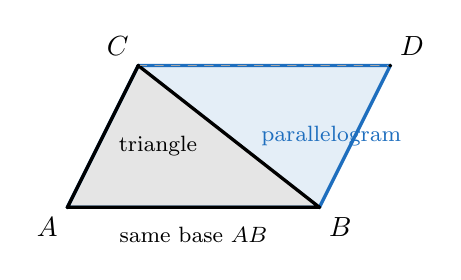
\begin{tikzpicture}[scale=1.0, line cap=round, line join=round]
  \definecolor{euclidblue}{RGB}{30,110,190}
  \coordinate (A) at (0,0);
  \coordinate (B) at (3.2,0);
  \coordinate (C) at (0.9,1.8);
  \coordinate (D) at (4.1,1.8);
  \fill[euclidblue!12] (A)--(B)--(D)--(C)--cycle;
  \fill[gray!20] (A)--(B)--(C)--cycle;
  \draw[very thick, euclidblue] (A)--(B)--(D)--(C)--cycle;
  \draw[very thick] (A)--(B)--(C)--cycle;
  \draw[gray!70, dashed] (C)--(D);
  \foreach \p/\pos in {A/below left,B/below right,C/above left,D/above right}{
    \fill (\p) circle (0.025);
    \node[\pos] at (\p) {$\p$};
  }
  \node[font=\footnotesize] at (1.6,-0.35) {same base $AB$};
  \node[euclidblue, font=\footnotesize] at (3.35,0.9) {parallelogram};
  \node[font=\footnotesize] at (1.15,0.78) {triangle};
\end{tikzpicture}
\end{center}


\begin{proof}[Professional Standard Proof]
\LRAProofBodyStart
Let parallelogram $ABDC$ and triangle $ABC$ have the same base $AB$ and lie
between the same parallels. Draw the diagonal $BC$ of the parallelogram. The
diagonal divides the parallelogram into two triangles on equal bases and in
the same parallels. These two triangles coincide in area by the earlier
parallel-area comparison.

One of those two triangles is the given triangle $ABC$. Hence the whole
parallelogram consists of two equal copies of that triangle, so the
parallelogram is double the triangle.
\end{proof}

\begin{proof}[Detailed Learning Proof]
\LRAProofBodyStart
Look at the diagonal. It cuts the parallelogram into two triangular halves.
Because opposite sides of the parallelogram are parallel, the two halves have
matching bases and matching altitude between the same parallel lines. Euclid
therefore treats them as equal in area. The parallelogram is the two halves
together, while the given triangle is one half.
\end{proof}

\begin{remark*}[Proof structure]
Cut the parallelogram by a diagonal, compare the two triangular halves, and
read the whole parallelogram as two equal copies of the triangle.
\end{remark*}

\begin{dependencies}
\begin{itemize}
  \item \hyperref[def:euclid-parallel-straight-lines]{Parallel straight lines}
  \item \hyperref[def:euclid-quadrilateral-classes]{Quadrilateral classes}
  \item \hyperref[ax:euclid-common-notion-coinciding-things-equal]{Euclid Common Notion IV}
\end{itemize}
\end{dependencies}

\clearpage
